%% This is an example first chapter.  You should put chapter/appendix that you
%% write into a separate file, and add a line \include{yourfilename} to
%% main.tex, where `yourfilename.tex' is the name of the chapter/appendix file.
%% You can process specific files by typing their names in at the 
%% \files=
%% prompt when you run the file main.tex through LaTeX.
\chapter{Background}

%% TODO I feel like I'm restating myself here?
Global climate change is `expected to increase the frequency and intensity of
floods'~\cite{ahernGlobalHealthImpacts2005}. Developing urban areas that are
undergoing unchecked development and rising population regularly experience
flooding~\cite{chanFloodRiskAsia2012}.  Nowhere is this more apparent than
in South and Southeast Asia, where the severity of floods has been increasing
over the past several decades~\cite{tortiFloodsSoutheastAsia2012}.

Of the world's 33 mega-cities with population over 10 million, over 60 percent
are located in developing Asian
Countries~\cite{unitednationsdepartmentofeconomicandsocialaffairsWorldCities20162016}.
These cities face a looming crisis as flood risk increases, but there are also
unique opportunities for risk mitigation. Megacities are characterized by high
population density, which leads to an increase in economic damages and loss of
life during flood events, but it also means that there are large numbers of
citizens that have disaster information they would like to share with
others~\cite{chanFloodRiskAsia2012}.

\section{History of Disaster Informatics} One of the best known and earliest
work in disaster informatics was John Snow's use of maps to find the source of
the 1857 Cholera outbreak in London\cite{rogersJohnSnowData2013}. This example
is taught to all students of epidemiology and illustrates the need
not only for up to date information, but for systems that ease the
analysis of this information. In John Snow's case, the map was the technology
that allowed him to visualize the spread of the disease and effectively take
action that ended the outbreak; however, the computer revolution has drastically
changed the way that scientists and responders analyze disaster information.
John Snow used mapping technology to track the spread of disease, but now
researchers are using artificial intelligence to predict cholera outbreaks
before they happen~\cite{radinskyMiningWebPredict2013}.

%% this needs to get moved somewhere else, but I'm not sure where...
In more recent times, the need for Information Technology (IT) in disaster
management has been clear since the mid 1980s when computers became user
friendly enough to be used during
disasters~\cite{universityTerminalDisastersComputer1986}.

Now many Emergency Operations Centers (EOCs) use Geographic Information Systems
(GIS), inventory control systems, and online messaging systems among other
technology in order to organize spatial data and analyze disaster information.
For example, Mozambique used an integrated disaster management system to provide
early warning during the 2007  Zambezi floods, while Guatemala's inventory
management helped to curb government bribes~\cite{aminDataNaturalDisasters2008}.
While some systems have helped some regions to better respond to disasters,
researchers have often stated that `there are many reasons to remain skeptical
about the idea that technology will provide a panacea for emergency management
problems'~\cite{tzemosUseGISFederal1995, tierneyFacingUnexpectedDisaster2001,
perryNaturalDisasterManagement2007}. A number of potential negative effects
associated with disaster management technology have been identified: the
primarily the potential of information overload and the dissemination of
incorrect and outdated
information~\cite{quarantelliProblematicalAspectsInformation1997,
flentgeDesigningContextAwareHCI}.

\subsection{Social Media and Disasters}
%% TODO is this in the right place??
The history of online communities is firmly linked to disasters. Internet
Relay Chat (IRC) was one of the first truly global online communication systems;
its adoption among internet connected citizens was `prompted by the First Gulf
War'~\cite{salazarHashtagsAnnotatedHistory2017}. Although radio and
television broadcasts were halted by the Iraqi army shortly after the invasion,
IRC communication continued for days afterward. IRC allowed users to communicate
about conditions on the ground, including the gulf war oil spill that grew to be
the largest oil spill in history~\cite{Timeline20Years2010}.

The history of social media and the hashtag is invariably linked to disaster
communication.  It was during the San Diego bush fires of 2007 that the hashtag
was first widely used on twitter~\cite{salazarHashtagsAnnotatedHistory2017}.

Quarantelli emphasized that  `management of hazards is fundamentally social in
nature and not something that can be achieved strictly through technological
upgrading'~\cite{tierneyFacingUnexpectedDisaster2001} yet social media brings
human behavior into a machine readable format that can be used to provide
further information during disasters.

Much work has been done in passively listening to social media streams in order
to better understand how disasters unfold and how humans use social media as a
communication tool during disaster events. Many of these studies use hand
labeled tweets in order to classify what kind of information people talk
about~\cite{alamTwitterTaleThree2018}.

Further work has evolved to using artificial intelligence methods to
automatically label new tweets using supervised learning. For example, Patrick
Meier's Haiti Crisis Map initially used volunteers to classify large number of
tweets, but his more recent projects focus on the use of AI for tackling big
data problems~\cite{meierDigitalHumanitariansHow2015}.
\subsection{Crowdsourcing vs. Passive Listening} 
As Patrick Meier points out in \textit{Digital Humanitarians}, `since
humanitarian organizations don't ask eyewitnesses on social media to report
information', they must passively wait and `rely on witnesses sharing relevant
information by chance'~\cite{meierDigitalHumanitariansHow2015}. Listening to
twitter data streams and hoping that someone posts relevant disaster information
is not always a winning strategy. One solution to this problem is to have paid
workers that collect information and enter it into disaster information systems
as in~\cite{aminDataNaturalDisasters2008}, which details how paid workers were
used to input data from citizens during the Mozambique floods of 2007; however,
this method is expensive and does not scale well. The same report states that
`data processing and consolidation [were] difficult' and that `the few data
entry clerks struggled to keep up'~\cite{aminDataNaturalDisasters2008}.

%% TODO not sure where to place this section?
\section{The Riskmap System}\label{chap1:riskmap}

	\subsection{Need for open data} Creating bespoke information systems at
	the beginning of disasters has been the
	norm~\cite{aminDataNaturalDisasters2008}; however this means that
	disaster response organizations must become acclimated with the system
	at the same time that they are dealing with disaster situations.
	Researchers have shown the need to create open sourced crowdsourced
	emergency systems that provide open
	data~\cite{avvenutiNeedOpeningCrowdsourced2018a}. The Riskmap system was
	created to fill that need.


	\begin{figure} 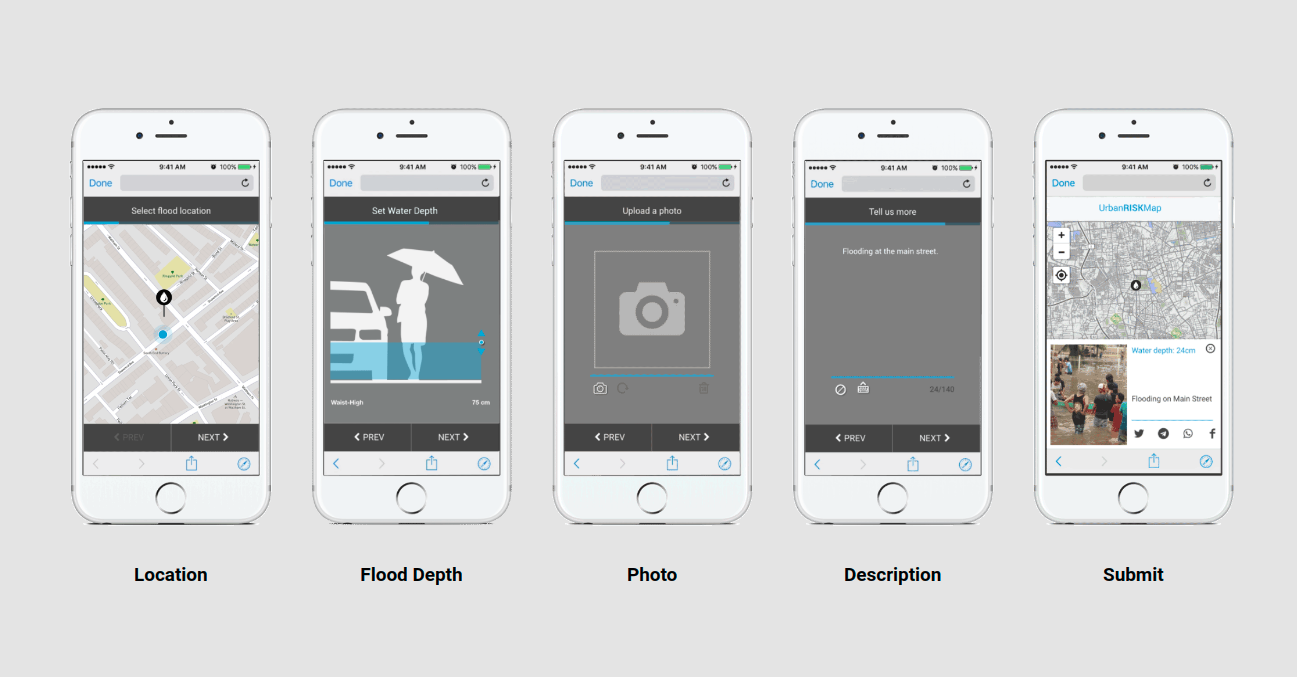
\includegraphics[width=\linewidth]{riskmap.png}
	\caption{Submitting a flood report card}\label{fig:cards} \end{figure}
	\subsection{System Overview} The Riskmap system alleviates the load on
	emergency managers by centralizing reports from many social media
	sources. It also makes it easy not only for reports to come into the
	response center, but also for emergency managers to indicate which areas
	of a city are most affected at any one time. The data gathered during an
	event is persistent and available under the Creative Commons license,
	which allows researchers to track the flood over time and pinpoint areas
	that are particularly vulnerable to flooding, thus fulfilling the need
	for open data~\cite{holdernessSocialMediaGeoSocial2015a}.

	Riskmap consists of many different social media bots that are actively
	filtering social media streams and looking for citizens that might be
	reporting flooding events, it then reaches out to those users and asks
	them to submit a flood report that consists of a GPS location, the
	estimated flood height at that location, a picture, and a textual
	description. The user interface for submitting these reports is shown
	in~\ref{fig:cards}. These reports are then displayed on a public map for other
	citizens to inform themselves. Furthermore, EOC personnel are able to
	access the Risk Evaluation Matrix (REM), a special dashboard that allows
	them to give even more information to citizens.

	The system has been in place in Jakarta and Chennai since 2016, and has
	seen hundreds of thousands of views during flood
	events~\cite{noveckOpinionElectionsWon2018, oct31ChennaiGetsRain}.

\section{Conquering Information Overload} It is not enough to create an advanced
system for consuming citizen reports, it is also necessary to ensure that this
system does not consume resources that are already scarce during a disaster
event, for example the time of emergency
workers~\cite{aminDataNaturalDisasters2008}. Furthermore, it is also important
to reduce the
resources needed to create insights because if analyzing data is too 
difficult, then decision makers will make decisions without having fully
analyzed the data~\cite{quarantelliUrbanVulnerabilityDisasters2003}.

Using computers to automatically make sense of disaster data has long
been a goal in disaster informatics, but only recently have machine
learning techniques become advanced enough to be implemented in production
emergency systems~\cite{meierDigitalHumanitariansHow2015}. Image
recognition algorithms can provide summaries of objects and scenes found
in user submitted photos~\cite{nguyenRapidClassificationCrisisRelated,
donahueDeCAFDeepConvolutional2013}. Natural language processing can
estimate the probability that a textual document is overall negative or
positive and thereby give EOCs a shorthand way to summarize thousands of
reports in short amounts of
time~\cite{nguyenRapidClassificationCrisisRelated,
nagyCrowdSentimentDetection2012}. Finally, ensemble learning methods can
learn relationships between disparate datasets and synthesize a single
result~\cite{mouzannarDamageIdentificationSocial2018}.

In this work we will experiment with different machine learning techniques
for image recognition, finally showing that transfer learning at the 
output layer can turn off the shelf multi---label  classification
algorithms into classifiers for flood image classification. For textual analysis, 
we will show the performance of bag of words, bigrams, and a combination of 
both techniques to classify report texts into heavy flooding/ no heavy flooding classes.
Flood height will first be assessed as a raw numerical feature but will then be 
joined with nearby reports through a one dimensional convolutional filter in order
to draw out temporal patterns. 

Finally, the output of these disparate techniques will be combined by using a 
small deep neural network. In order to allow better interpretability, the
most important labels from feature extraction machine learning algorithms are
presented to the user so that they can understand what drove the machine's
choice.

	// lay out problem statement for thesis
